% -*- coding: utf-8 -*-
\newpage
\section{Atomic Properties}

Atomic properties are computed only when explicitly requested by the user by
setting \texttt{AnalysisLevel} to \texttt{Extended} or \texttt{Full}. In these
cases, the calculation of the topology is followed by the evaluation of the
atomic properties:

\begin{lstlisting}[language=bash]
  QTAIM
    # [atomic properties / non-local properties]
    AnalysisLevel [Extended/Full]
  End 
\end{lstlisting}

\subsection{Atomic Dipole Moment}

The electronic contribution to the atomic dipole moment within
\gls{QTAIM} was already implemented in the \ams code.
However, the nuclear contribution was not previously included. As shown
in Equation~\ref{atomic_dipole}, the nuclear contribution can be computed
with the \gls{QTAIM} topology and atomic charges.

In the rare event that the topology fails for a specific ring, the
corresponding ring is excluded from the linear system used to compute the
nuclear contribution. The dimensions of the linear system are given by the
number of bonds (columns) and the number of atoms plus the number of rings
(rows).  Since the system is overdetermined, omitting a ring does not prevent a
solution from being obtained.

In the even less common case where the linear system cannot be solved, a
warning is issued in the output file and the nuclear contribution to the atomic
dipole moment is set to zero (\texttt{0.d0}). The system is solved using the
\texttt{DGELSS} \subroutine from \lapack, which handles both overdetermined and
underdetermined systems. It computes the minimum norm solution to a real linear
least squares problem: $\min || \underline{\underline{A}}\mathbf{x} -
\mathbf{b} ||$, using the singular value decomposition of
$\underline{\underline{A}}$.  The \texttt{info} flag returned by
\texttt{DGELSS} is checked to ensure successful resolution of the system, and
an additional safeguard is applied: if any component of the solution lies
outside the physically reasonable range of $-19.9$ to $+19.9$, the result is
discarded.

\newpage
A nuclear dipole contribution flagged as zero is internally interpreted
as a failure. In practice, no physical system should yield a zero
nuclear dipole contribution for all atoms, except in highly symmetric
molecules. Even in such cases, numerical precision typically produces
values fluctuating around positive and negative zero
rather than exact double-precision zeros. The proof of this is
provided in the Appendix~\ref{zero_nuclear_contribution}.

Because the calculation of the nuclear contribution draws upon both the
topological data and the atomic charges, generated by \texttt{LocalProperties}
and \texttt{AtomicProperties} respectively, it is invoked only once those two
\subroutines have terminated successfully. All three \subroutines are
dispatched from the total energy \subroutine, as summarised in
Algorithm~\ref{toten}.

% -*- coding: utf-8 -*-

\begin{algorithm}[h!]
  \SetNoFillComment
  % \tcc{src/toten/toten.f90}

  \tcc{Local properties}
  ADFAIMCriticalPoints()\;

  \tcc{The system is divided into blocks for parallelisation}
  \For {iblock $\gets 1$ \KwTo nblocks}{
     \If {skip\_block(iblock)}{
        $\mathbf{nextBlock}$
     }   
     \tcc{Atomic properties}
     \If {gQTAIM.atomic}{
        AssignAtomicBasinsForBlock() \tcp*{Map grid points to the attractors}
        UpdateAIMTerms() \tcp*{Properties computed by integrating $\rho$}
     }   
  }

  MergeValuesComputedInParallel()\;

  \tcc{When the local and atomic properties are computed, the nuclear and 
       (electronic + nuclear) dipole can be computed}
  \If {gQTAIM.atomic}{
     AIMdipole() \tcp*{nuclear dipole moment}
  }
  \caption{Total energy subroutine for the ADF Engine}
  \label{toten}
\end{algorithm}



\newpage
The \texttt{UpdateAIMTerms} \subroutine evaluates all atomic observables
that can be expressed as integrals of the electron density over a
\gls{QTAIM} basin; its control flow is given in
Algorithm~\ref{updateaimterms}.

% -*- coding: utf-8 -*-

\begin{algorithm}[h!]
  \SetNoFillComment

  % \tcc{src/adf/bader7/ADFBaderAnalysis.f90}
  \tcc{Symmetry}
  \For {no $\gets 1$ \KwTo nogr}{
    \tcc{For each gridpoint in the block}
    \For {i $\gets 1$ nblocksize}{
      \tcc{-1 means that the point is not a part of an attractor basin}
      \If {attLabel(i) > 0}{
        \tcc{Weight from the gridpoint}
        $\rho$ += $\rho$(i)$\times$weight(i)\;
        $\boldsymbol{\mu}_p$ += (coord\_block(i) - coord\_attractor(i))$\times\rho$(i)$\times$weight(i)\;
        \tcc{The rest of the properties computed by integration of $\rho$}
        \tcc{Quadrupole, laplacian, spin density, volume, Ts, Tsl, Tc}
      }   
    }   
  }

  \caption{Atomic properties computed by the integral of the density}
  \label{updateaimterms}
\end{algorithm}



Finally, \texttt{ADFdipole} assembles the atomic dipole moment by combining the
electronic obtained above, computing the nuclear contributions and adding they
two, as outlined in Algorithm~\ref{adfdipole}.

% -*- coding: utf-8 -*-

\begin{algorithm}[h!]
  \SetNoFillComment

  \tcc{Set the topological connection in a matrix}
  \tcc{no bond : 0; bond (A-B) : 1; bond (B-A) : -1}
  qbondmat $\gets$ topologicalConnection

  \tcc{Expand the linear system in case of rings}
  qbondmat $\gets$ overdetermineSystem(qbondmat, ringsInfo)\;

  \tcc{Solve the linear system A*x = B}
  chargeBonds $\gets$ lapack(qbondmat, atomicCharges)\;
  check\_values(chargeBonds) \tcp*{Physically realistic values?}

  \tcc{Nuclear dipole moment contribution}
  \For {i $\gets 1$ \KwTo nAttractors}{
    \For {j $\gets 1$ \KwTo nAttractors}{
      \If {bonded(i,j)}{
        $\boldsymbol{\mu}_c$(i) += (coord\_attractors(i) - coord\_bcp(i,j))$\times$ chargeBonds(i,j)\;
      }
    }
  }
  \tcc{Nuclear \& Electronic dipole moment}
  $\boldsymbol{\mu}_t$ $\gets$ $\boldsymbol{\mu}_c - \boldsymbol{\mu}_p$

  \caption{Atomic properties computed by the integral of the density}
  \label{adfdipole}
\end{algorithm}



\newpage
\subsection{Polarisability}

The calculation of atomic polarisabilities within \gls{QTAIM} requires a
numerical approach, these properties are obtained from finite-field
calculations. This involves performing separate \gls{SCF} calculations for each
applied external electric field configuration. To manage this workflow, two
parallel implementations were developed. The first, based on \plams, automates
the sequence of calculations externally. The second, integrated directly into
the \ams driver, was designed to provide seamless compatibility with the
\gls{GUI}.

In both cases, the required single-point calculations are executed in parallel
to improve efficiency. The \plams implementation, however, is limited in that
it cannot export the results in a format suitable for graphical visualisation.
The \ams driver implementation overcomes this limitation by writing the
computed polarisabilities not only to the standard output, but also to the
binary files used by the \ams graphical interface, enabling direct
visualisation of the atomic polarisability tensors.

\begin{figure}[h]
  \centering
  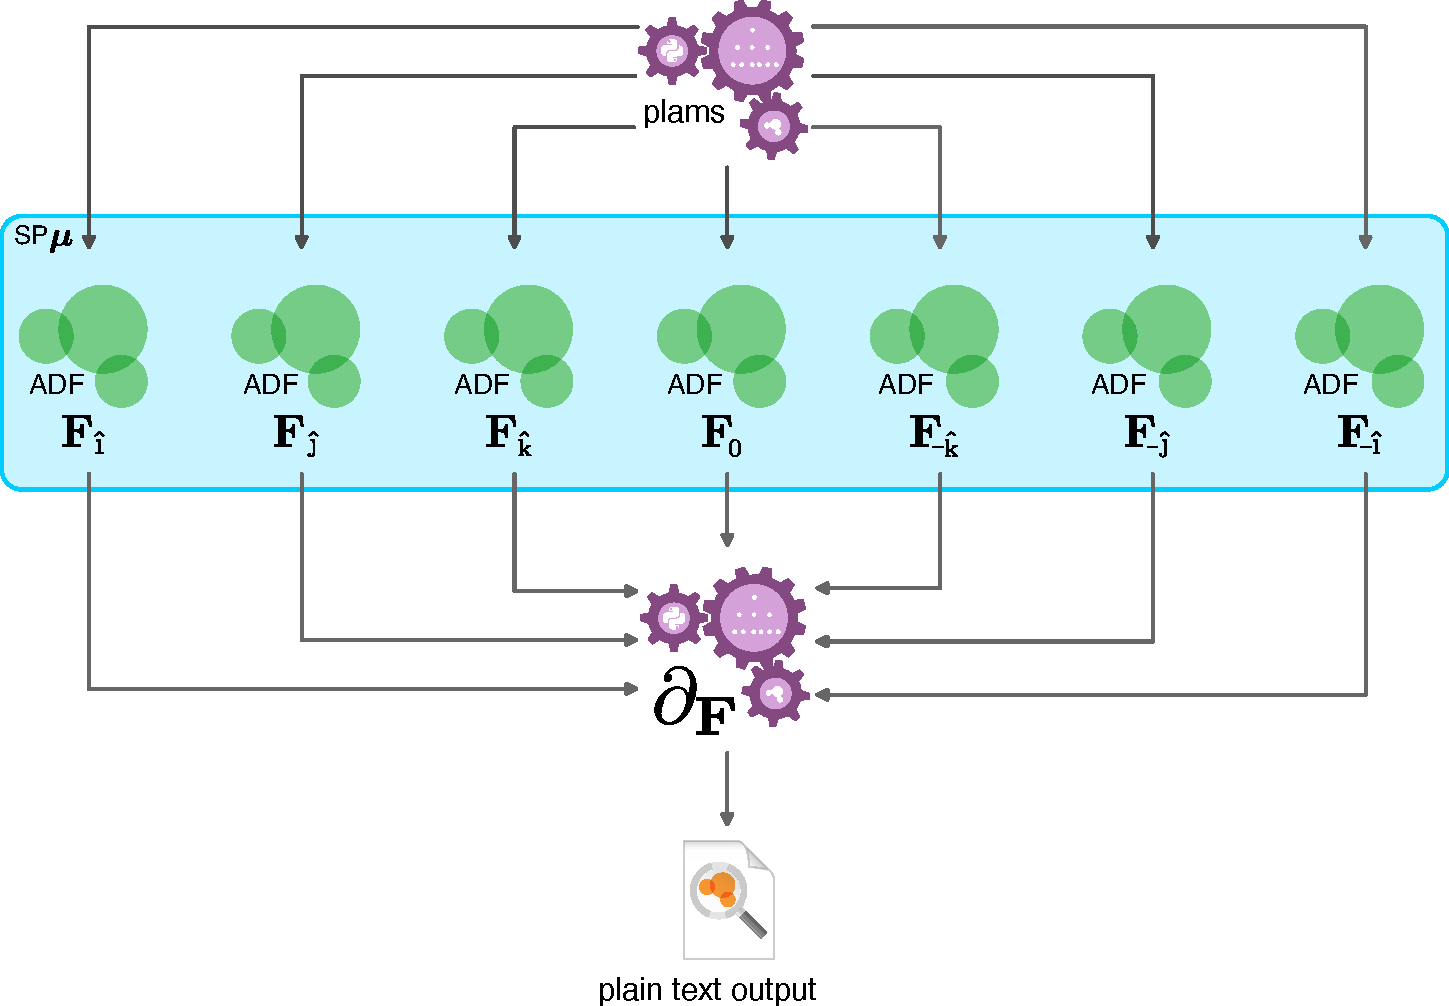
\includegraphics[width=0.8\textwidth]{diagramas/pola_diagram.pdf}
  \caption{Workflow of the polarisability calculation by \plams.}
  \label{polarisability_workflow}
\end{figure}

\newpage
To simplify the use of the \plams workflow, we encapsulated the procedure in a
\python class. As a result, the full set of calculations needed for the
polarisability of a system can be launched easily as well as the numerical
derivaties. The next summarised \python code illustrates the implementation:

% -*- coding: utf-8 -*-

\begin{lstlisting}[language=Python, style=mystyle, basicstyle=\tiny]
class DipoleMomentJob(MultiJob):
    """Dipole moment with an electric field in (x,y,z,-x,-y,-z) directions.

    Attributes:
        molecule:             The molecule to calculate the dipole moment for.
        common_settings: Common settings for all jobs.
        directions:            Directions of the electric field.
        eField:                Electric field values.
    """
    def __init__(self, molecule, common_settings, directions, eField, **kwargs):
        """Initializes the DipoleMomentJob with molecule, settings, directions,
           and electric field."""
        MultiJob.__init__(self, children=OrderedDict(), **kwargs)
        # Code omitted for brevity
        # self.molecule = molecule; self.eField; self.setup_jobs()

    def setup_jobs(self):
        # Code omitted for brevity

    def collect_results(self) -> Tuple[np.ndarray, np.ndarray]:
        """Collects and returns the dipole moments."""

  # Inicialize and run the DipoleMomentJob's in the PLAMS workflow

  dipole_job = DipoleMomentJob(molecule=mol,
                                              common_settings=adfsettings,
                                              directions=directions, eField=eField)
  dipole_job.run()

  # Collect the results
  dipole, atom_charge = dipole_job.collect_results()
  # Numerical derivatives
  pol_tensor = np.zeros((natoms, 3, 3)) 
  for j in range(natoms):
      pol_tensor[j,:,:] = (dipole[:3,j,:] - dipole[3:6,j,:])/(2.0*eFieldmag)

\end{lstlisting}



\newpage

The \plams recipe can operate either from a plain \texttt{xyz} geometry
file or from the results of a prior \adf\ calculation. In both cases, the
magnitude of the applied electric field defaults to $0.01$~a.u.\ (input in
V/\AA), unless overridden by the user through the \texttt{eFieldmag}
keyword.

When a previous \adf\ calculation is provided, the recipe automatically
adopts the same level of theory as that calculation. If the atomic
properties for the electric field-free system are already computed in the \adf output,
the workflow bypasses their recomputation and proceeds directly to launch
the six additional single-point calculations required for the finite-field
analysis.

When an \texttt{xyz} file is used as the starting point, the workflow
assigns a default level of theory of M06-2X/TZ2P. This ensures a consistent,
reasonably accurate description for systems.

\subsubsection{Example usage}

A typical invocation of the recipe is illustrated below. The workflow is
executed directly from the terminal, the calculation with the \texttt{xyz} file
is performed with optional argument used to modify the electric field for the
calculation (0.005~a.u.).

\begingroup
\setstretch{0.95}
\lstset{style=terminal, numbers=none, basicstyle=\tiny, escapeinside={(*@}{@*)}}
% > drwxr-xr-x  3 user  group     -  Aug 12 14:32 .
% > drwxr-xr-x 14 root  root      -  Aug 12 09:15 ..
\begin{macterminal}[vcastor@aragorn - bash]
$ ls -l
> total 7
> -rw-r--r--  1 user  group   10k  Jan 20 11:13 QTAIMpol.py
> -rw-r--r--  1 user  group   150  Aug 11 14:32 water.xyz
> -rwxr--r--  1 user  group   580  Aug 11 14:32 water.run
> -rw-r--r--  1 user  group   76k  Aug 11 14:32 water.out
> drw-r--r--  8 user  group   405  Aug 11 14:36 water.results
$ # from a previous calculation
$ $AMSBIN/plams QTAIMpol.py -v resultsdir=./water.results
$ # from scratch  
$ $AMSBIN/plams QTAIMpol.py -v xyzfile=./water.xyz -v eFieldmag=0.26
$ ls -la *poldip
> -rw-r--r--  1 user  group  1.3k  Aug 11 15:39 water.poldip
\end{macterminal}
\lstset{style=mystyle}
\endgroup

\newpage
\subsection{Excited States}

As shown in Equation~\ref{mu_ct}, the change in dipole moment,
$\Delta\boldsymbol{\mu}$, between the ground and an excited state can be
evaluated. In \adf, molecular orbitals and their corresponding grid coordinates
can be extracted for each block (grid region), enabling the computation of
$\Delta\boldsymbol{\mu}$ within \gls{QTAIM}.

Since the loop over all grid points, points already labelled with an
attractor in the ground state, the decomposition of the excited-state dipole
moment reduces to assigning each contribution to its corresponding atomic
basin. 

Although minor differences may exist between the ground- and excited-state
topologies, adopting the ground-state partition significantly accelerates the
calculation of the excited-state dipole moment while preserving accuracy. A
condensed version of the \fortran implementation is provided below.

\newpage

% -*- coding: utf-8 -*-

\begin{lstlisting}[language=Fortran, style=mystyle, basicstyle=\tiny]
      rhop = 0._kreal; rrhop = 0._kreal; rrhon = 0._kreal
      ! The system is divided into blocks for parallelisation
      iblock_ : do iblock = 1, gDims%nblock
         if (skip_block(G, iblock)) cycle iblock_
         call get_block(G); call calc_bas_block(BAS, G, bas0) ! Parallel stuff
         if (BAS%local_num == 0) cycle iblock_

         allocate(moCoef(BAS%local_num, nocc+nvir), bas0tmp(G%npoints, BAS%local_num))

         ! get the occupied and virtual orbitals
         do i = 1, BAS%local_num
            iao                    = BAS%global_index(i)
            bas0tmp(:, i)       = bas0(:, iao)
            moCoef(i, 1:nocc) = occao(iao, :)
            moCoef(i, nocc+1:nocc+nvir) = virao(iao, :)
         enddo
         ! Optimised matrix multiplication
         ! (SCM BLAS [Basic Linear Algebra Subprogram] implementation)
         call SCMgemm(bas0tmp, moCoef, mo) ! mo = bas0tmp * moCoef

         ! Connect the grid to the QTAIM grid atom mapper
         call GetGridAtomMap(aimGridAtomMapper, attLabel)

         ! update the coordinates
         ! replicate G%w along dimension 2 to match shape of G%coord
         coordw = G%coord*spread(G%w, 2, 3)
         ! squere of the MO coefficients
         mo2 = mo*mo

         ! The integrals start here; k is the index for every point in the block
         do k = 1, blocksize; if (AttLabel(k) .gt. 0) then ! Skip points with no label
            atom = AttLabel(k)
            ! [[ \int r\rho_+ = \langle \varphi_a | \hat{r} | \varphi_a \rangle ]]
            do i = 1, nocc; do j = 1, 3
               rrhop(atom) = rrhop(atom) + sum(mo2(:,i)*coordw(:,j))
            enddo; enddo
            ! [[ \int r\rho_- = \langle \varphi_i | \hat{r} | \varphi_i \rangle ]]
            do i = 1, nvir; do j = 1, 3
               rrhon(atom) = rrhon(atom) + sum(mo2(:,i+nocc)*coordw(:,j))
            ! [[ \int \rho_+  = \langle \varphi_a | \varphi_a \rangle ]]
            enddo; enddo
            rhop(atom) = rhop(atom) + sum(mo2(:,1:nocc))
         endif; enddo
      end do iblock_
\end{lstlisting}



